\documentclass[11pt]{beamer}

\usepackage[T1]{fontenc}
\usepackage{tikz}
\usepackage[quiet]{mathspec}
\usepackage{ifthen}

\usetikzlibrary{matrix,arrows.meta}

% The base16 colour scheme?
\definecolor{sbase03}{HTML}{002B36}
\definecolor{sbase02}{HTML}{073642}
\definecolor{sbase01}{HTML}{586E75}
\definecolor{sbase00}{HTML}{657B83}
\definecolor{sbase0}{HTML}{839496}
\definecolor{sbase1}{HTML}{93A1A1}
\definecolor{sbase2}{HTML}{EEE8D5}
\definecolor{sbase3}{HTML}{FDF6E3}
\definecolor{syellow}{HTML}{B58900}
\definecolor{sorange}{HTML}{CB4B16}
\definecolor{sred}{HTML}{DC322F}
\definecolor{smagenta}{HTML}{D33682}
\definecolor{sviolet}{HTML}{6C71C4}
\definecolor{sblue}{HTML}{268BD2}
\definecolor{scyan}{HTML}{2AA198}
\definecolor{sgreen}{HTML}{859900}

\definecolor{Tropiteal}{RGB}{0,168,198}
\definecolor{TealDrop}{RGB}{64,192,203}
\definecolor{WhiteTrash}{RGB}{249,242,231}
\definecolor{AtomicBikini}{RGB}{174,226,57}
\definecolor{FeebleWeek}{RGB}{143,190,0}
\definecolor{ICantExpress}{RGB}{28,20,13}
\definecolor{Marty}{RGB}{250,42,0}

\colorlet{ColourBase}{Tropiteal}
\colorlet{ColourHl1}{Marty}
\colorlet{ColourHl2}{FeebleWeek}
\colorlet{ColourHl3}{TealDrop}
\colorlet{ColourDark}{ICantExpress}
\colorlet{ColourDark2}{Tropiteal}


\usetheme{metropolis}

\setbeamercolor{alerted text}{%
  fg=bazelGreen
}

\setbeamercolor{example text}{%
  fg=mLightBrown
}

\setbeamercolor{frametitle}{%
  use=normal text,
  fg=normal text.bg,
  bg=bazelGreen
}

\lstset{%
  basicstyle=\ttfamily\lst@ifdisplaystyle\fontsize{9pt}{9pt}\selectfont\fi,
  keywordstyle=\color{sgreen}, identifierstyle=\color{sblue}, 
  commentstyle=\color{sbase1}, stringstyle=\color{sorange},
  numberstyle=\color{sviolet}, showstringspaces=false,  
  breaklines=true,
  tabsize=5,
}

\lstalias[]{gnumake}[gnu]{make}

% --------------------------- %
% tikz settings and libraries %
% --------------------------- %

\usetikzlibrary{calc,intersections,positioning,matrix,chains,scopes}
\usetikzlibrary{decorations.pathmorphing,decorations.pathreplacing,shapes}
\usetikzlibrary{decorations.text,backgrounds}
\usetikzlibrary{arrows.meta,bending}

% -------------------- %
% Additional functions %
% -------------------- %

\DeclareMathOperator{\real}{Re}
\DeclareMathOperator{\tr}{Tr}
\newcommand{\tikzmark}[1]{\tikz[overlay,remember picture] \coordinate (#1);}

% To get "eqnarray" centred alignment
% See: http://tex.stackexchange.com/a/102845/39313
\newcommand*\centermathcell[1]{\omit\hfil$\displaystyle#1$\hfil\ignorespaces}


\author{Jonas Rylund Glesaaen}
\title{Hadronic spectrum calculations in the quark-gluon plasma}
\institute{
  Swansea University \\
  In collaboration with G. Aarts, C. Allton, S. Hands, \underline{B. Jäger}, %
  J. Skullerud
}
\date{July 27th 2018}

\begin{document}

\begin{frame}[plain]
  \maketitle
\end{frame}

\begin{frame}{Talk overview}
  \setbeamertemplate{section in toc}[sections numbered]
  \tableofcontents[hideallsubsections]
\end{frame}

\section{Introduction}

\begin{frame}
  \frametitle{Baryons at finite temperature}

  Although mesons have been thoroughly studied at finite temperatures, baryons
  have not been given nearly the same attention

  \begin{itemize}\setlength\itemsep{1em} 
    \item They have definite parity: $P_{\pm} \mathcal{O}_B(x) = \mathcal{O}_B(x)$
    \item Experimentally accessible results
    \item Important for model builders
    \begin{itemize}
      \item Quark models, e.g. hadron resonance gas
      \item Verification of thermodynamic models
    \end{itemize}
  \end{itemize}

\end{frame}

\begin{frame}
  \frametitle{More broken symmetries...}

  In nature baryon parity is a \alert<1>{broken} symmetry
  %
  \begin{alignat*}{99}
    m_{\{uud\}^{1/2^+}} &{}\equiv{}& \centermathcell{m_{N}} &{}={}& 0.939\; \mathrm{GeV} \\
    m_{\{uud\}^{1/2^-}} &{}\equiv{}& \centermathcell{m_{N*}} &{}={}& 1.535\; \mathrm{GeV}
  \end{alignat*}

  \vspace{.3cm}

  Similar to other broken symmetries, what happens to this one as we increase
  temperature and enter the deconfined phase?

  \vspace{.5cm}

  \uncover<2->{
    Previous studies by \alert{FASTSUM}:
    {\par\centering{}
    1502.03603, 1703.09246, 1710.00566, ...\par}
  }

\end{frame}

\begin{frame}
  \frametitle{Open questions}

  \begin{itemize}\setlength\itemsep{1em} 
    \item Does parity restoration happen at $T_c$?
    \item How does hadron content effect parity restoration?
    \item Is there a flavour hierarchy in the deconfinement transition?
    \item How does $m_{\pi}$ affect parity restoration?
  \end{itemize}
\end{frame}

\section{Method}

\begin{frame}
  \frametitle{Lattice setup - Gen2l ensembles}

  Results produced with the FASTSUM "\alert<1>{Gen2l}" ensembles\\
  (lattice parameters by the HadSpec collaboration)

  \begin{itemize}
    \item $N_f = 2 + 1$ dynamical quarks, Wilson-Clover action
    \item Anisotropic action: $a_s = 0.1227(8)\, \text{fm},\;a_s / a_t = 3.5$
    \item $m_{\pi} = \alert<1>{236\; \text{MeV}}$, $m_s = \text{\emph{physical}}$
  \end{itemize}

  \begin{center}
    \begin{tabular}{c|cccccccccc}
      $N_t$ & $256$ & $48$ & $40$ & $36$ & $32$ & $28$ & $24$ & $20$ & $16$ \\ \toprule
      \tikzmark{temp}\color{ColourDark2!50}$T / T_c$ & %
      \color{ColourDark2!50}\scalebox{0.8}{$0.12$} & %
      \color{ColourDark2!50}\scalebox{0.8}{$0.63$} & %
      \color{ColourDark2!50}\scalebox{0.8}{$0.76$} & %
      \color{ColourDark2!50}\scalebox{0.8}{$0.84$} & %
      \color{ColourDark2!50}\scalebox{0.8}{$0.95$} & %
      \color{ColourDark2!50}\scalebox{0.8}{$1.09$} & %
      \color{ColourDark2!50}\scalebox{0.8}{$1.27$} & %
      \color{ColourDark2!50}\scalebox{0.8}{$1.52$} & %
      \color{ColourDark2!50}\scalebox{0.8}{$1.90$} \\
      $N_{\mathrm{cfg}}$ & \scalebox{0.8}{$750$}\tikzmark{hadspec} & %
      \scalebox{0.8}{$500$}\tikzmark{low1} & \scalebox{0.8}{$500$}\tikzmark{low2} & %
      \scalebox{0.8}{$500$}\tikzmark{low3} & \scalebox{0.8}{$500$}\tikzmark{low4} & %
      \scalebox{0.8}{$1000$} & \scalebox{0.8}{$1000$} & \scalebox{0.8}{$1000$} & %
      \scalebox{0.8}{$1000$}
    \end{tabular}
  \end{center}

  \vspace*{-5mm}

  \nointerlineskip
  \begin{uncoverenv}<2>
    \begin{tikzpicture}[overlay,remember picture]
      \draw[{Stealth}-] ([shift={(-2mm,1mm)}] temp) %
        .. controls +(-.8cm, 0) and +(-.8cm, 0) .. %
        +(0,-1.5cm) %
        node[right,scale=0.8,align=left] {Have to be \alert{checked}, numbers from Gen2 ensembles};
    \end{tikzpicture}
  \end{uncoverenv}
  \begin{uncoverenv}<3>
    \begin{tikzpicture}[overlay,remember picture]
      \draw[{Stealth}-] ([shift={(-2mm,-1mm)}] hadspec) %
        .. controls +(0, -0.5cm) and +(-2cm, 0) .. %
        +(2cm,-0.5cm) %
        node[right,scale=0.8,align=left] {By the \alert{HadSpec} collaboration};
    \end{tikzpicture}
  \end{uncoverenv}
  \begin{uncoverenv}<4>
    \begin{tikzpicture}[overlay,remember picture]
      \coordinate (target) at ([shift={(1cm, -0.6cm)}] low4);
      \draw[{Stealth}-] ([shift={(-2mm,-1mm)}] low1) %
        .. controls +(0, -0.5cm) and +(-4cm, 0) .. (target);
      \draw[{Stealth}-] ([shift={(-2mm,-1mm)}] low2) %
        .. controls +(0, -0.5cm) and +(-3cm, 0) .. (target);
      \draw[{Stealth}-] ([shift={(-2mm,-1mm)}] low3) %
        .. controls +(0, -0.5cm) and +(-2cm, 0) .. (target);
      \draw[{Stealth}-] ([shift={(-2mm,-1mm)}] low4) %
        .. controls +(0, -0.5cm) and +(-1cm, 0) .. (target)
        node[right, scale=0.8] {\alert{Still generating}};
    \end{tikzpicture}
  \end{uncoverenv}
\end{frame}

\begin{frame}{Lattice setup - baryon correlation functions}

  Use the following baryon interpolation functions:
  %
  \begin{align*}
    \chi_{N,\gamma} &= \epsilon^{abc} u^{a}_\gamma (u^b_{\alpha} (C \gamma_5)_{\alpha\beta} d^c_{\beta}) \\
    \chi_{\Delta^+,\gamma,\mu} &= \epsilon^{abc} \big( %
      2 u^{a}_\gamma (u^b_{\alpha} (C \gamma_{\mu})_{\alpha\beta} d^c_{\beta}) + %
    d^{a}_\gamma (u^b_{\alpha} (C \gamma_{\mu})_{\alpha\beta} u^c_{\beta})\big) \\
    \chi_{\Delta^{++},\gamma,\mu} &= \epsilon^{abc} u^{a}_\gamma (u^b_{\alpha} (C \gamma_{\mu})_{\alpha\beta} u^c_{\beta}) \\
  \end{align*}

  \vspace*{-8mm}

  for all baryons that can be constructed with from them having flavour content
  using $\{u, d, s, c\}$

  \begin{itemize}
    \item $N$, $\Delta_{s/c}$, $\Sigma_{s/c}$, $\Sigma^*_{s/c}$, $\Xi_{s/c}$, $\Omega_{s/c}$
  \end{itemize}

  Sinks and sources smeared with Gaussian smearing to extract ground states

\end{frame}

\section{Results}

\begin{frame}
  \frametitle{Parity and correlation functions}

  Due to charge conjugation symmetry (at $\mu = 0$)

  \begin{equation*}
    G_{\pm}(\tau, \mathbf{p}) = - G_{\mp}(1/T - \tau, \mathbf{p})
  \end{equation*}

  Thus the correlation function is a sum of forward moving
  $\text{parity}^+$ states and backwards moving $\text{parity}^-$ states

\end{frame}

\begin{frame}
  \frametitle{Correlation functions}

  \vspace*{-8mm}
  \begin{center}
    \hspace*{-8mm}
    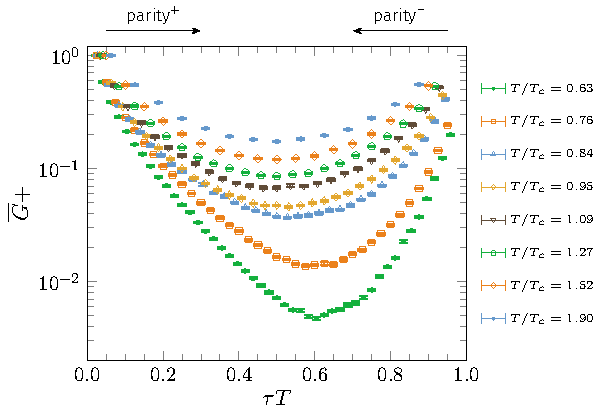
\includegraphics[width=1.1\textwidth]{plots/correlator_symmetry.pdf}
  \end{center}

\end{frame}

\begin{frame}
  \frametitle{Parity channels - nucleon}

  \begin{center}
    \hspace*{-10mm}
    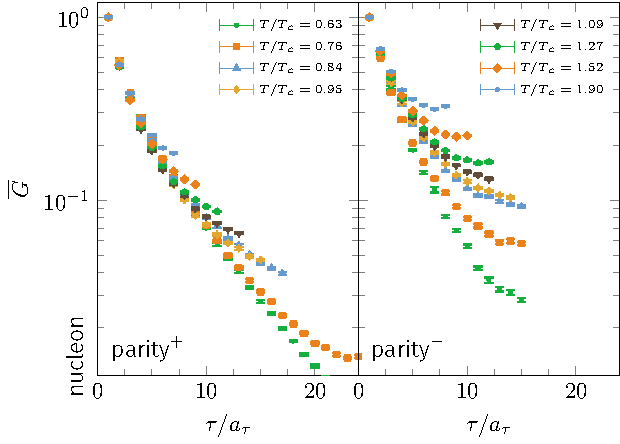
\includegraphics[width=\textwidth]{plots/correlator_nucleon.pdf}
  \end{center}

\end{frame}

\begin{frame}
  \frametitle{Parity channels - $\Delta^{+}$ particle}

  \begin{center}
    \hspace*{-10mm}
    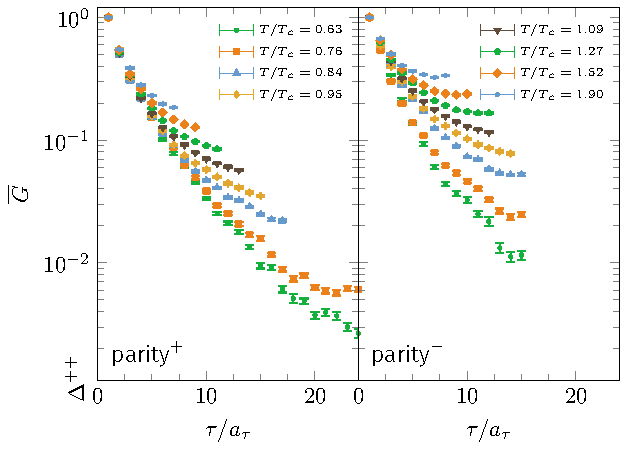
\includegraphics[width=\textwidth]{plots/correlator_delta.pdf}
  \end{center}

\end{frame}

\begin{frame}
  \frametitle{Parity channels - $\Omega$ particle}

  \begin{center}
    \hspace*{-10mm}
    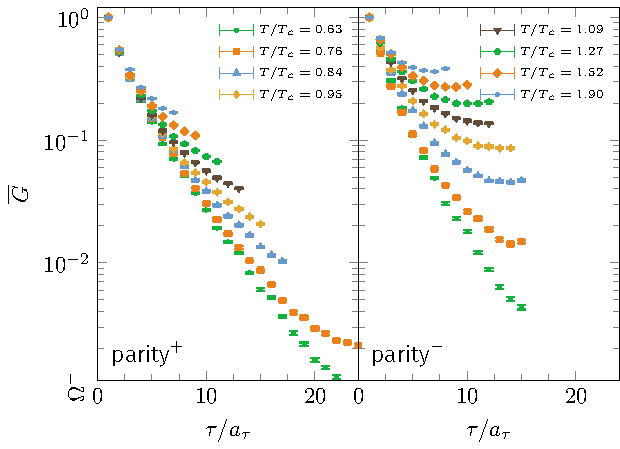
\includegraphics[width=\textwidth]{plots/correlator_omega.pdf}
  \end{center}

\end{frame}

\begin{frame}
  \frametitle{Parity channels - $\Omega_c$ particle}

  \begin{center}
    \hspace*{-10mm}
    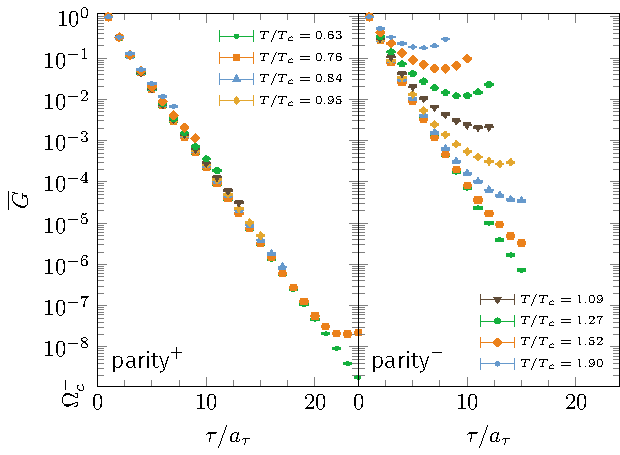
\includegraphics[width=\textwidth]{plots/correlator_omega_c.pdf}
  \end{center}

\end{frame}

\begin{frame}
  \frametitle{Symmetry restoration parameter - the R parameter}

  \begin{equation*}
    R(\tau) = \frac{%
      G_+(\tau) - G_+(1/T - \tau)
      }{%
      G_+(\tau) + G_+(1/T - \tau)
    }
  \end{equation*}

  \begin{itemize}
    \item $R(\tau) \neq 0 \Leftrightarrow \text{no parity doubling}$
    \item $R(\tau) = 0 \Leftrightarrow \text{parity doubling}$
  \end{itemize}

  \vspace{5mm}

  The summed ratio is a quasi-order parameter \scalebox{0.8}{(as we will see)}
  %
  \begin{equation*}
    R = \frac{%
      \sum_n R(\tau_n) / \sigma^2(\tau_n)
      }{%
      \sum_n 1 / \sigma^2(\tau_n)
    }
  \end{equation*}

\end{frame}

\begin{frame}
  \frametitle{The R-factor - $S = 0$}

  \vspace{6mm}
  \begin{center}
    \hspace*{-5mm}
    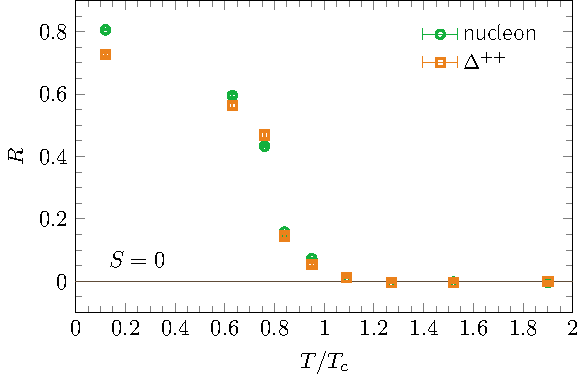
\includegraphics[width=\textwidth]{plots/sumR_nucleon.pdf}
  \end{center}

\end{frame}

\begin{frame}
  \frametitle{The R-factor - $S = -1$}

  \vspace{6mm}
  \begin{center}
    \hspace*{-5mm}
    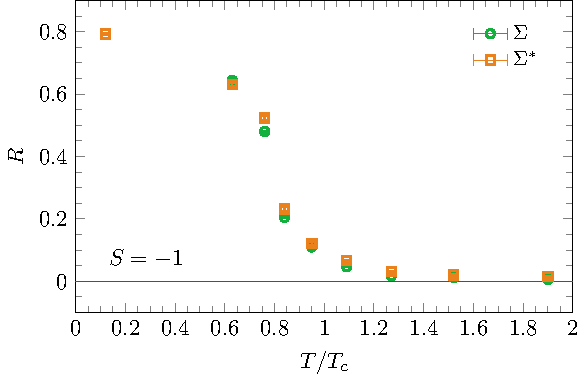
\includegraphics[width=\textwidth]{plots/sumR_s1.pdf}
  \end{center}

\end{frame}

\begin{frame}
  \frametitle{The R-factor - $S = -2$}

  \vspace{6mm}
  \begin{center}
    \hspace*{-5mm}
    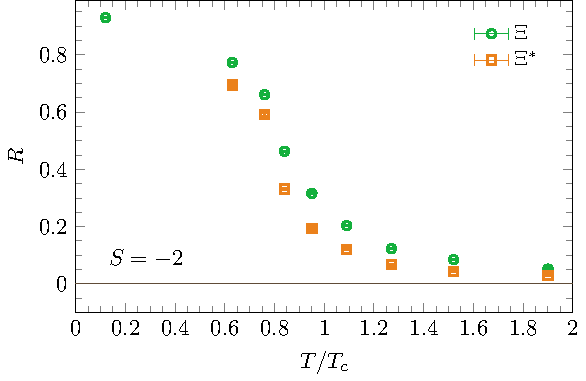
\includegraphics[width=\textwidth]{plots/sumR_s2.pdf}
  \end{center}

\end{frame}

\begin{frame}
  \frametitle{The R-factor - $S = -3$}

  \vspace{6mm}
  \begin{center}
    \hspace*{-5mm}
    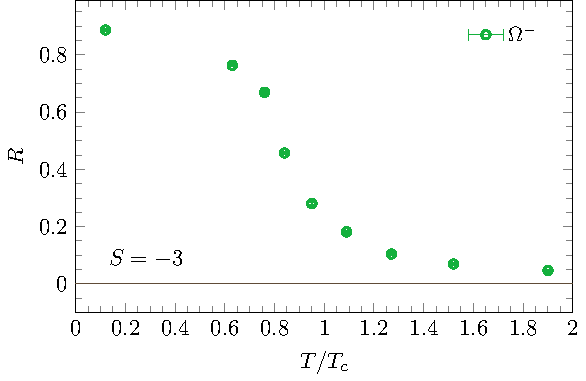
\includegraphics[width=\textwidth]{plots/sumR_omega.pdf}
  \end{center}

\end{frame}

\begin{frame}
  \frametitle{The R-factor - $\Omega_c$ particle}

  \vspace{6mm}
  \begin{center}
    \hspace*{-5mm}
    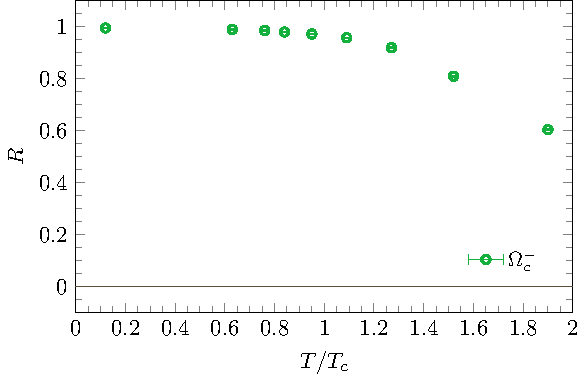
\includegraphics[width=\textwidth]{plots/sumR_omega_c.pdf}
  \end{center}

\end{frame}

\begin{frame}
  \frametitle{The R-factor - comparison with previous ensemble}

  \vspace{6mm}
  \begin{center}
    \hspace*{-5mm}
    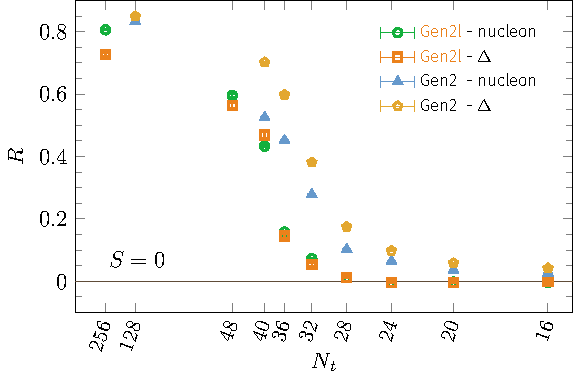
\includegraphics[width=\textwidth]{plots/sumR_compare.pdf}
  \end{center}

\end{frame}

\section{Future work}

\begin{frame}
  \frametitle{Still a lot more to be done}

  {\bfseries\color{ColourBase}Study just getting started}
  \begin{itemize}
    \item More thorough look at the masses and correlators
    \item Spectral reconstruction analysis
    \item Susceptibility calculations
  \end{itemize}

  \vspace{.5cm}

  {\bfseries\color{ColourHl1}Planned future ensembles}
  \begin{itemize}
    \item Generation \alert{2P} \uncover<2->{(physical quark masses)}
    \item Generation \alert{3}\hphantom{P} \uncover<3->{(higher anisotropy)}
  \end{itemize}
\end{frame}

\section{openQCD-FASTSUM}

\begin{frame}
  \frametitle{openQCD-FASTSUM}

  {\bfseries\color{ColourBase}Two major features}
  \begin{itemize}
    \item Anisotropic lattice actions
    \item Stout link smearing
  \end{itemize}

  + AVX512 optimisations courtesy of the SA2C

  \vspace{.5cm}

  \begin{uncoverenv}<2->
    {\bfseries\color{ColourHl1}Future development plans}
    \begin{itemize}
      \item Library/back-end interface
      \item Unit testing and CI
    \end{itemize}

    \begin{center}
      \begin{tikzpicture}
        \node[draw, font=\color{ColourHl1}, inner sep=3mm] {\url{https://fastsum.gitlab.io}};
      \end{tikzpicture}
    \end{center}
  \end{uncoverenv}

\end{frame}

\begin{frame}[standout]
  Questions?
\end{frame}



\end{document}
